%% Author_tex.tex
%% V1.0
%% 2012/13/12
%% developed by Techset
%%
%% This file describes the coding for rsproca.cls

\documentclass[]{rsos}%%%%where rsos is the template name

\usepackage{lineno}
\linenumbers

\usepackage[T1]{fontenc}
\usepackage[utf8]{inputenc}


% tightlist command for lists without linebreak
\providecommand{\tightlist}{%
  \setlength{\itemsep}{0pt}\setlength{\parskip}{0pt}}

% From pandoc table feature
\usepackage{longtable,booktabs,array}
\usepackage{calc} % for calculating minipage widths
% Correct order of tables after \paragraph or \subparagraph
\usepackage{etoolbox}
\makeatletter
\patchcmd\longtable{\par}{\if@noskipsec\mbox{}\fi\par}{}{}
\makeatother
% Allow footnotes in longtable head/foot
\IfFileExists{footnotehyper.sty}{\usepackage{footnotehyper}}{\usepackage{footnote}}
\makesavenoteenv{longtable}


\usepackage{float}
\usepackage{booktabs}
\newcommand{\beginsupplement}{ \setcounter{table}{0}     \renewcommand{\thetable}{S\arabic{table}}\setcounter{figure}{0} \renewcommand{\thefigure}{S\arabic{figure}}}

%%%% *** Do not adjust lengths that control margins, column widths, etc. ***

%%%%%%%%%%% Defining Enunciations  %%%%%%%%%%%
\newtheorem{theorem}{\bf Theorem}[section]
\newtheorem{condition}{\bf Condition}[section]
\newtheorem{corollary}{\bf Corollary}[section]
%%%%%%%%%%%%%%%%%%%%%%%%%%%%%%%%%%%%%%%%%%%%%%%

\begin{document}


%%%% Article title to be placed here
\title{Combination of field and experimental data together with computational models reveal cognitive mechanisms behind cleaner fish behaviour}

\author{
Andrés E. Quiñones$^{1}$,
Zegni Triki$^{2}$,
Redouan Bshary$^{1}$}

\address{
  $^{1}$Institute of Biology, University of Neuchâtel, Neuchâtel, Switzerland\\
  $^{2}$Department of Zoology, Stockholm University, Stockholm, Sweden}
%%%% Subject entries to be placed here %%%%
\subject{
Behavioural ecology,
Cognitive ecology,
Animal behaviour}

%%%% Keyword entries to be placed here %%%%
\keywords{
learning,
cleaners,
behaviour,
bayesian statisitics,
mutualism}

%%%% Insert corresponding author and its email address}
\corres{
  AE. Quiñones\\
  e-mail: \href{mailto:andreseqp@gmail.com}{\nolinkurl{andreseqp@gmail.com}}
}

%%%% Abstract text to be placed here %%%%%%%%%%%%
\begin{abstract}
While it is generally straightforward to quantify individual performance in cognitive experiments, identifying the underlying cognitive processes remains a major challenge. Often, different mechanistic underpinnings yield similar performances, and Lloyd Morgan's cannon warrants acceptance of the simpler explanation. Alternatively, when the different mechanisms interact with environmental conditions, variation in performance across environments might allow to statistically infer the mechanism responsible. However, to do this it is necessary to have quantitative predictions for the different candidate mechanisms. Here, we use a set of computational models to get quantitative predictions from alternative learning mechanisms, and using Bayesian statistics fit the model parameters to performance data. We used experimental data on performance in an ephemeral reward task by wild-caught cleaner fish \emph{Labroides dimidiatus}, as well as cleaner and client fish densities from the locations of capture. The task can in principle be solved by estimating future consequences of an action, or by perceiving the removal of the ephemeral reward as psychological punishment (negative reinforcement). We found that a model where cleaners only estimate the future consequences of their actions explains best which cleaner fish relative abundances cause the fish to develop a preference for an ephemeral food source. This model also yields performances that can be considered the result of locally optimal decision-rules, in contrast to the negative reinforcement model. We argue that the combination of computational models with data is a powerful tool to infer the mechanistic underpinning behind cognitive performance.
\end{abstract}
%%%%%%%%%%%%%%%%%%%%%%%%%%%

\providecommand{\EndFirstPage}{%
}

\maketitle

\hypertarget{introduction}{%
\subsection{Introduction}\label{introduction}}

Disentangling the mechanistic underpinnings of behaviour
is typically done under controlled conditions in a laboratory setting. However,
controlled laboratory conditions often mask the inter and intra-specific
variation that arises in the interaction between mechanisms and
environmental variation. From a evolutionary perspective, mechanisms
are likely selected because of how they allow individuals to respond to
environmental variation. For example, biological market theory predicts that
the exchange rate of goods and/or services traded between cooperative
partners adjusts to the law of supply and demand, when individuals have
some degree of partner choice \citep{noe_Biological_1995a}.
Supply and demand conditions, which typically
depend on the abundance of the species involved, certainly vary in time
and space. Therefore, natural selection should
favour the ability to flexibly adjust decisions and behavioural output to
current market conditions. Indeed, such adjustments have been repeatedly
documented \citep{axen_Signalling_1996}. In animals, an obvious general candidate
mechanism for the strategic adjustment is the cognitive machinery. However,
it is not clear which cognitive mechanisms allow individuals to adjust their
behaviour to the varying conditions. As adjustments to changes in
market conditions have been documented in a great variety of species with
highly variable brain anatomies, the question arises to what extent mechanisms
beyond basic associative learning may be involved.

One example of strategic adjustment in a biological market is the marine
cleaning mutualism involving the cleaner fish \emph{Labroides dimidiatus} and
`client' fish. Client fish seek cleaner fish services at their territory
(so-called ``cleaning station'') and offer themselves as food patches
to get their ectoparasites removed, which provides cleaners
with food and clients with improved health \citep{waldie_LongTerm_2011, ros_Does_2011, triki_Effects_2016, demaire_Reduced_2020}.
Given the capacity of some client fish to swim larger distances and
access multiple cleaning stations while others access the only cleaning
station at their territory, it is crucial to categorize clients as
either ``visitors'' or ``residents'', respectively. During cleaning interactions,
a cleaner fish often face a choice between a visitor and a resident client
seeking its cleaning services simultaneously. Visitors have the option
to switch to another cleaner fish if being made to wait, while residents
must wait for inspection. Indeed,
visitors have been observed to use their partner choice option in that
way \citep{bshary_Choosy_2002}, which may explain why cleaners give
visitors service priority in a field study in the Red Sea
\citep{bshary_Cleaner_2001a}.

When researchers aimed at testing wild-caught cleaner fish, as
well as individuals from other species, abilities
to prioritize visitor over resident clients in a lab-based paradigm,
they used Plexiglas plates of different colours and shapes offering same
amount of food as surrogates for visitor and resident clients.
One plate is made to behave like a resident, i.e.~it remains until
the cleaner fish had eaten off it. The other plate was made to behave
like a visitor, i.e.~it is removed if not inspected first.
Cleaners learned to prefer the visitor plate and
hence obtained the double amount of food \citep{bshary_Asymmetric_2002}.
Furthermore, adult cleaner fish outperformed various primates as well as rats and
pigeons in this original version of the biological market task
\citep{salwiczek_Adult_2012, zentall_Early_2017}; yet the African grey
parrots solve this task as well \citep{pepperberg_Can_2014}. Given that primates
are known to readily distinguish
between one and two reward units if presented in more conventional ways
\(\color{red}{\text{ref}}\), this raises the question:
what makes the task difficult for most non-cleaners?

Recent research on the cognitive tool kit needed to solve the ephemeral
reward task has used a broad approach as proposed by Shettleworth
\citep{shettleworth_Cognition_2009}, who defined cognition as including
all ways in which animals acquire information
through the senses, process, retain and decide to act on it.
Indeed, perception of relevant cues is of major importance
for individual performance. For example, some animals find relevant
information in the plates
\citep{wismer_Cuebased_2019} while others find it in the food
\citep{pretot_Comparative_2021, pretot_Comparing_2016}. However, identifying
cues as salient is not the only challenge of the ephemeral reward task,
as revealed by proximate learning models. Such models allow varying the
cognitive tool kit and to evaluate which minimal kit is necessary to solve
the task at hand (e.g. \citep{dubois_Model_2021}). Applied to the ephemeral
reward task, learning models showed that basic reinforcement learning does
not suffice to solve the ephemeral reward task \citep{prat_Modelling_2022, quinones_Reinforcement_2019}.
This is particularly so when models assume the more complex natural
situation in which cleaner fish not only face resident-visitor pairs but also
visitor-visitor and resident-resident pairs, as well a resident alone or
a visitor alone. To be able to give visitors priority over residents,
cleaners need to be able to assess a client's value separately for the
three possible scenarios (alone, paired with a fish with the
same strategic option, paired with a fish with the alternative strategic option)
\citep{quinones_Reinforcement_2019}. The ability to distinguish and value differently
one stimulus alone from compound versions of it has been termed
configurational learning, or chunking,
or segmentation (see references in \citep{prat_Modelling_2022}).

To solve the ephemeral reward task, cleaners need to account for
the future consequences of current decisions. In the model by
Quiñones \emph{et al.} \citep{quinones_Reinforcement_2019}, this could be achieved in
two non-mutually exclusive ways: through low temporal discounting of
future effects, also termed `chaining' \citep{enquist_Power_2016}; and/or
through perceiving a visitor client leaving as psychological punishment
(i.e.~as a negative reinforcer). Low temporal discounting is when
individuals include in their valuation of an action the reward effects
that this will have in the future. This is done by combining in a single
valuation the reward obtained in the current time with all the reward that
comes after, discounting for how far in the future reward
is accrued. `Chaining' the reward of these different time steps allows
individuals to take actions that increase the long-term reward at the sacrifice
of short term considerations \citep{enquist_Power_2016}. Even though, `chaining'
can be readily implemented computationally in learning models
\citep{enquist_Power_2016, sutton_Reinforcement_2018}, cognitively it seems to be
a complex adaptation \citep{suddendorf_Evolution_2007}. On the other hand,
using client behaviour as a negative reinforcer is in principle
easier to implement. Negative reinforcement is part of the ubiquitous
learning mechanism termed operant conditioning \citep{thorndike_Animal_1898, skinner_Behavior_1938}. Thus, standard logic of
Lloyd Morgan's cannon demands that operant conditioning as the simpler
explanation is to be accepted by default. Ideally, the two mechanisms should
be evaluated in light of how well they explain the available data.

Over the last decade, our team tested over a hundred of wild-caught
cleaner fish in the exact same paradigm of of the ephemeral reward
task \citep{salwiczek_Adult_2012, wismer_Variation_2014, triki_Decrease_2018, triki_Biological_2019, triki_Brain_2020}. These fish often come from
different reef locations around the study field site at Lizard Island,
Great Barrier Reef in Australia. Further investigation of the local
eco-sociological conditions revealed that cleaner and client
fish population densities have a substantial impact on cleaner fish
performance in the task. Cleaner fish from reef sites with relatively
low densities were more likely to fail at solving the task \citep{triki_Biological_2019, triki_Decrease_2018, wismer_Variation_2014}. The explanation for this pattern
is twofold. First, low cleaner fish population densities imply
low supply and high demand for cleaning services.
Under such conditions, there are fewer occasions under
which failing to give priority to a visitor translates to an empty
cleaning station. Second and also related to the state of the cleaning market,
visitor clients at low cleaner fish population densities
are less likely to exert their partner choice options
and are hence more likely to wait for inspection if not given cleaning
priority \citep{triki_Brain_2020}. In the absence of partner choice
cleaners should not give priority to visitors any more.

The interplay between the underling cognitive machinery and
local ecological conditions apparently generate the documented variable
performance among individuals of the same species.
Our approach of fitting the computational model to the empirical data on
fish densities and cleaner fish censuses and performance
in the ephemeral reward task aimed at: (i), determining which
mechanism cleaner fish use to incorporate future consequences of current
decisions by testing whether operant conditioning, chaining, or a combination
of both best explains their performance; (ii) determining whether the
two mechanisms differed with respect to the ecological conditions
that are likely to cause high versus low performance in the
ephemeral reward task. Additionally, we assessed which mechanism
yields optimal performance patterns. Relying on the logic of
biological market theory, we predicted
that appropriate performance is to show low preference for visitors under low
local cleaner-to-client ratio.

\hypertarget{methods}{%
\subsection{Methods}\label{methods}}

\hypertarget{the-model}{%
\subsubsection{The model}\label{the-model}}

The model consists of a set individual-based simulations where
individuals, representing cleaners, face a series of choices
between two options, which simulate the natural conditions
of the cleaning market. Individuals experience a series
of discrete time points in which they face different `states',
defined by the number and category of client fish (visitor or residents)
inviting for cleaning services. There are six possible states:
zero clients, one resident, one visitor,
resident-resident, visitor-visitor, and resident-visitor.
The probability of each state is largely determined by the relative
abundance of cleaner fish, residents and visitors, but to some degree by
cleaner fish choices when it faces the resident-visitor combination.
This is because residents are willing to queue for cleaning service;
while visitors leave the queue (with a certain probability) when made to wait.
Individuals obtain a fixed reward from cleaning a client fish
regardless of the category. Every time individuals face and make a choice
they update the probability of making that same choice. The update is
based on the difference between the expected reward and the obtained
reward (prediction error) \citep{sutton_Reinforcement_2018, rescorla_Theory_1972}. Given the new information, the update is carried
in the direction that leads to more reward being obtained, given
the new information. In the long run, the probability of choosing a visitor
over a resident converges in the model. To which probability the model
will converge depends on the relative abundance of cleaners, visitors
and resident; as well as on the probability of visitors leaving the
cleaning station when made to wait. Further details of the model
implementation can be found in Quiñones \emph{et al} \citep{quinones_Reinforcement_2019}.

The model shows that agents need to find a mean
to incorporate future consequences of current choices. In the model,
this could be achieved with either of two parameters that could
also work together. First, \(\gamma\) measures how
much individuals include future rewards in their decision updates. If
\(\gamma=0\), individuals only use the immediate reward obtained from a
cleaning interaction. As \(\gamma\) increases individuals include more the
reward obtained from the subsequent choices. That amounts to calculating
and using for decision making the future expected rewards of an action.
Second, \(\eta\) measures how much individuals include in their reward the
fleeing behaviour of visitor as a negative component. Both of
these parameters allow individuals to use in their estimates the future
effects of their choices.

\hypertarget{empirical-data}{%
\subsubsection{Empirical data}\label{empirical-data}}

The empirical data were collected between 2010 and 2019 always during
the austral winter months June to August from a total of five
study reef sites (Corner Beach-CB, Horseshoe-HS, Mermaid Cove-MC,
Northern Horseshoe-NHS, and The Crest-TC) at Lizard Island
(\(14.6682° S, 145.4604° E\)), Great Barrier Reef, Australia.
The data consist of three sets: fish censuses, field
observations of cleaner-client interactions to quantify the probability
of visitors leaving if made to wait, and the
performance of wild-caught cleaner fish in the ephemeral reward test.
In total, we have twelve site/year data sets for fish censuses and
corresponding performance in the lab test. Thus, some sites were sampled more
than once. To estimate the population density of cleaner fish
and their clients at a given site in
a given year, Triki \emph{et al.} \citep{triki_Biological_2019} used a series of ten
transects of \(30m\) each. Observers swam along the transect lines placed on
the reef and first counted the visible large-bodied adult fish
(species with total length \(TL \geq 10cm\)) including cleaner fish
on a width of \(5m\), and then on the
return individuals of small-bodied fish species (\(TL < 10 cm\))\\
on a width of \(1 m\)
(see Triki et al.~2018 for further details on fish censuses data collection).
We then scaled the counts of cleaner fish, small-bodied,
and large-bodied clients fish densities per \(100 m^2\).
From the study by Triki \emph{et al} \citep{triki_Biological_2019}
cleaner fish and large-bodied client populations densities were
highly correlated, and only the former
was hence used in the analyses as representative of both measures.

The field observation data consisted of video recordings/encodings of the
cleaner-client cleaning interactions. There were videos from eight
cleaners per site/year of a duration of \(30 min\) each. Triki \emph{et al}
extracted information from every event wherein a visitor client
was made to wait in favour of another client (visitor or resident), and noted
whether or not the visitor left or queued for the cleaning service
\citep{triki_Biological_2019, triki_Brain_2020}.

The cognitive performance data was from a total of 120 cleaners
(10 individuals per 12 site/year) tested in the
ephemeral reward task \citep{triki_Biological_2019, triki_Brain_2020}. Authors
housed all captured cleaners individually in glass aquaria
( \(62cm \times 27cm \times 37 cm\) ) and provided them
with PVC pipes (\(10 cm \times 1 cm\)) as shelters.
The task consisted of exposing the cleaner fish to substitute
models of client fish in the form of two \emph{Plexiglas} plates offering the
same amount of food (one item of mashed prawn). The two plates differed
in colour and pattern (horizontal green stripes or vertical pink stripes)
but had equal size (\(10 cm \times 7 cm\)). Importantly, the two plates played
different roles as either a visitor (ephemeral food source) or
resident (permanent food source). That is, if a cleaner fish inspected the
resident plate first, the experimenter withdrew the visitor plate out of
the aquarium as a consequence. Choosing first the visitor plate,
however, granted access to both plates. The equal size of the plates
forced cleaner fish to learn to give service priority to the visitor plate
based solely on the behaviour-cue of the plates rather than size-cue
\citep{wismer_Cuebased_2019}. Triki \emph{et al.} \citep{triki_Biological_2019, triki_Brain_2020}
tested the fish for a maximum of 200 trials with 20 trials a day, 10 trials
in the morning and 10 trials in the afternoon. They randomized and
counterbalanced the plates' spatial location (i.e.~left or right)
between trials. Similarly, they counterbalanced the plates' decoration
(colour and pattern) and the plates' role (visitor or resident) between the
tested fish. In the original studies, once a fish reach a learning criterion,
that is, performing significantly above chance level (\(> 50%
\), \(p-value ≥ 0.05\)),
they passed to a reversal version of the task where the roles of the
visitor/resident Plexiglas plates were swapped (see Triki et al.~2019, 2020).
Here, we used instead a subset of these data in order to have an idea on
cleaner fish preferences for the visitor plate, even if they do not reach
the learning criterion within 200 trials. To do so, we first extracted the
trial-by-trial outcomes from the last two session (20 trials) of those who
never reached the learning criterion for visitor plate
(\(N = 45\) cleaner fish).
For those who reached the learning criterion at some point during the
test and passed to a reversal phase, we extracted the trials-by-trial
outcomes from the last session (10 trials) before passing to reversal
and the last 10 trials they were exposed to in the test
(\(N = 75\) cleaner fish).

\hypertarget{statistical-analysis}{%
\subsubsection{Statistical analysis}\label{statistical-analysis}}

The aim of the analyses is to fit the key model parameters
\(\gamma\) and \(\eta\), to the empirical data from Triki \emph{et al.}
\citep{triki_Biological_2019, triki_Brain_2020} to test whether each or
a combination of these effects is a better explanation for the pattern
seen in the data. We used the ecological variables: cleaners, visitor clients,
resident clients abundances and visitor clients leaving probability,\\
as input to the models. As response variable we used cleaners'
preference for visitor over residents in the ephemeral reward task.
Finally, we used the preference for visitors resulting from the
model simulations as the prediction for the response variable.
We kept all other parameter values used for the model simulations constant,
see Table \ref{tab:param}.

To capture with the model the relationship between the ecological
variables and cleaner fish preferences for visitors we need to scale
the absolute population densities of cleaner fish from the empirical data
to a measure of relative abundances that captures client visitation patterns.
This is because in the model, relative abundances of clients
define not only the probability of residents and visitors,
but also how often the cleaning station is empty (e.g.~there are no
clients to be cleaned). The frequency with which clients visit the station
is another variable, which in nature may vary among different client species
depending on their ectoparasite loads. We do not have field estimates
for species-specific parasite loads, especially not as a function of site.
In order to control for these aspects, we computed a measure of relative
cleaner fish abundance for each reef site relative to
absolute abundances and multiplied it
by a scaling constant that changes the range of the variable. This scaling
constant is hence meant to capture variation in the market conditions driven
partly by cleaner fish abundance. We fitted the value of the scaling constant as
part of the statistical inference. As for the visitor and resident
abundances we computed a relative measure with respect to the
total client abundance, and weighted that by the rescaled relative absence
of cleaners (\(1-\text{relative cleaner abundance}\)). Thus, all three measures
of relative abundance sum up to 1, and can be used in the model as a proxy
for the probability of having different options in the cleaning station.
Note that we introduced the scaling constant to control for variation that
is not captured by the model; its parameter distribution does not offer
biological insights.

Once we calculated the relative abundances, we obtained predictions from
the model for each one of the locations and ran the Markov Chain. We started the
chain with random values for the parameters of interest, then ran the
computational model once for every reef site using as input the ecological
explanatory variables. The model outputs the probability of choosing the visitor
for each location \(p_i\), where \(i\) is the index for the 12 locations. Assuming a
binomial distribution, the probability that each of the cleaner fish 20 choices
in the ephemeral reward task was generated by the model
is given by \(\binom{n}{k_ij}p^{k_{ij}}_i (1-p_i)^{n-k_{ij}}\);
where \(k_{ij}\) is the number of times that cleaner fish \(j\) in reef site \(i\)
chose the visitor over the resident; and \(n=20\) (due to our choice of using 20
choices per cleaner fish). By taking the natural logarithm and summing over all
the cleaner fish and reef sites we obtained the log-likelihood of the data
given the model and parameters. We then proposed a new set of parameters drawn
from a uniform distribution centred around the old parameter set. The amplitude
of the uniform distribution used for each parameter can be found in Table
\ref{tab:param}. Subsequently, we ran the model and calculated the likelihood
with the new parameter set. We then used the ratio of the two likelihoods to
choose which parameter set to keep. New parameter sets with a higher likelihood
than the old set replaced old ones, and those with a lower likelihood replaced
current ones with a probability equals to the log-likelihood ratio.
Given that we only used the likelihoods in the decision, we used a
uninformative prior. Once we decided whether the new parameter set replaces
the old one, we ran the model again to sample the likelihood
distribution of the parameter set. We then started
the cycle again by proposing a new set of parameters, and repeated
the process for \(1e^5\) steps. We ran 5 independent chains,
discarded the first \(1000\) samples of each chain as burn in,
and after that we kept 1 in every 100 samples to avoid autocorrelation.
The collection of parameters sets kept in
all chains approximates the posterior distribution. We coded the model
as well as the fitting algorithm in \emph{c++}, the diagnostics and visualization
in R \citep{rcoreteam_Language_2021}. All codes are accessible at
\(\color{red}{\text{include citation}}\)

To compare the fit of the three alternative models, we used the
distribution of pseudo \(R^2\) proposed by Mcfadden \citep{mcfadden_Conditional_1974}.
Mcfadden's pseudo \(R^2\) is a standard measure of fit for logistic regression.
In that context, \(pseudo-R^2\) uses the log-likelihood of the data given
the model, relative to the log-likelihood of the data given a
model without covariates, as a measure of fit. Our
model is not a logistic regression, therefore we measured the \(pseudo-R^2\) in
relation to the log-likelihood of a model
with parameters \(\gamma\) and \(\eta\) set to zero. This in practice
amounts to a model that has neutral preference between the two options.
We computed the pseudo \(R^2\) for all the samples of the posterior from
the MCMC. Thus, we used these distributions of pseudo \(R^2\)'s as a measure of
fit.

\hypertarget{results}{%
\subsection{Results}\label{results}}












Figure \ref{fig:post} panels a,b and c show the posterior distributions
of the parameter values of the full model, which includes both chaining
and operant conditioning (negative reward). Posterior distributions show the probability
density (y axis) of the estimated parameter values (x axis). Notably,
the bulk of the posterior distribution for the parameter tuning negative
reward (\(\eta\) panel b) was around zero. Thus, the shape of the posterior
and its credible intervals suggest the absence of negative reward to be
well supported by the data. As for \(\gamma\), the confidence intervals
also includes zero, but the mode of the posterior is around 0.5. Thus,
we ran the analysis setting \(\eta\) to zero. Figure \ref{fig:post} panels
d and e, show the posterior distributions of the two parameters
estimated. Not surprisingly, under a model without negative reward, the
distribution of \(\gamma\) shifted to higher values. Under the new model,
the estimates of \(\gamma\) did not include zero and the distribution was
centred around \(0.5\). In panel f of figure \ref{fig:post}
we show the distribution of \(pseudo-R^2\) calculated using
samples from the posterior distributions shown before,
as well as from a model with negative reward but without
future reward. Note, \(pseudo-R^2\) can have negative values, which is when
the log-likelihood of the model is lower than that of a model that
triggers neutral preferences. Even though, the peak of the three
\(pseudo-R^2\) distributions was not very different, the model with only
future reward produced a distribution of \(pseudo-R^2\) where more values
were positive (to the right of black line in Fig. \ref{fig:post} f). This
shows that, accounting for variation in the parameter estimates, the
model with only future reward gives a better fit to the data, despite
having one parameter less.




















Figure \ref{fig:pred} shows predictions from the two models,
one including chaining and operant conditioning (upper panels) and
one with only chaining (lower panels). On the
left, the colour coded contour shows the prediction of the model for
combinations of cleaner fish abundance (x axis) and visitor leaving
probability (y axis). Predictions were generated by running the model
using the mode of the posterior distributions as the parameter values,
and varying systematically cleaner fish abundance and visitor leaving
probability. Colour of the dots on top of the contour show the average
frequency with which cleaner fish chose the visitor plate in their last
20 experimental trials. Each dot corresponds to a reef-site/year of
data collection with a combination of cleaner fish abundance
and visitor leaving probability. Panels
on the right show how close the observed values for the probability of
choosing the visitor (y axis) were from the predictions of the models (x
axis). The black line represents the perfect fit between observed and
predicted values. Bars show the variation in predicted values using 100
samples from the posterior distribution. Despite having one more
parameter varying, the full model
gave a lower fit to the data than the model without negative reward.
In the supplementary material, we also show predictions from
model with only negative reward, excluding future rewards (\(\gamma=0\),
Fig. \ref{fig:nogamma}), provides a lower fit than either of the ones
presented in the main text.

The main reason for chaining and operant conditioning to give different
predictions is the way that cleaner fish relative abundance influences the
preference for the visitor clients. Visitor leaving probability has a
similar positive effect on the probability of choosing the visitor
clients on all three models (Fig. \ref{fig:pred}, \ref{fig:nogamma}). In
contrast, cleaner fish relative abundance has a different effect in the
model with only chaining, compared to the other two models,
full model and only operant conditioning. In the model
with only chaining, only intermediate cleaner fish abundance triggers a
preference for the visitor clients (Fig. \ref{fig:pred} c). In models
with negative reward, both intermediate and low cleaner abundance
triggered a preference for the visitor. (Fig. \ref{fig:pred} a,
\ref{fig:nogamma}).

\hypertarget{discussion}{%
\subsection{Discussion}\label{discussion}}

In this study, our main aim was to unravel which of two potential
cognitive mechanisms, chaining of events, operant conditioning,
or their combination, best explains wild-caught cleaner fish
performance in the ephemeral reward task, while accounting for their
ecological conditions. To evaluate the merits of each of these two mechanisms
separately and combined, we considered cleaner fish performance
in the lab test to have its origin from the these fish apply
in their natural environment. That is, individuals that
solved the task already had a preference for
visitors clients, and generalized this rule to the lab conditions
once being familiar with the task.

While all three models captured well the positive relation between visitor
leaving behaviour and cleaner fish performance in
the market task \citep{triki_Biological_2019}, only the chaining mechanism
predicted that cleaner fish performance in the task should be low in
habitats with low cleaner-to-client ratios, regardless of the
visitor leaving probability. In contrast, models including
negative reward predicted the highest performance in the ephemeral
reward task when relative cleaner fish abundance is low, particularly
together with high probability of visitor leaving (Fig. \ref{fig:pred}).
Low relative cleaner fish abundances mean the market has an excess of demand for
cleaning services. In the models, this translates to a cleaning station
that is frequently full. Thus, when a visitors leaves, it is likely that the
cleaner fish will have access to another client in the next step. Therefore,
there will not be much difference in future reward between choosing
a visitor and a resident, and cleaners will not develop a preference for the
visitor in these conditions. On the other hand, the effect of negative reward
on cleaner fish preference is the opposite, as in a busy cleaning station, to
that of chaining. cleaner fish will get more often the resident-visitor
state and will develop a preference for the visitor faster.
At high cleaner fish abundances, the resident-visitor state
becomes so rare that neither mechanism is very efficient
at generating a preference for visitors. When facing the resident
visitor choice it is still be best to choose the visitor; however,
the learning machinery will not be able to develop this preference
efficiently. Overall, the models suggest that chaining is the cognitive
mechanism that allows cleaner fish to adaptively adjust to their
biological market ecological conditions.

Our results support chaining as the more plausible mechanism behind the
intra-specific variation in cleaners' performance. This suggest
that chaining could be under positive selection. In the standard ephemeral
reward task, however, food amount and quality are equal in the
two Plexiglas plates. Since our computational models simulate this aspect of
the task, choosing visitors over residents at low cleaner fish abundances
does not diminish the amount of food/reward in the models.
On the other hand, a cleaner fish committed to visitors might find it more difficult
to include in its decision making other variables, like parasite load
and/or mucus quality \citep{roche_Client_2021}. Indeed, in the absence of
market effects, both field observations and laboratory experiments also
using simultaneous two choice options, show that cleaner fish base their
decision-making on other cues such as the mucus quality and the amount of food.\\
\citep{triki_Fluctuations_2019, grutter_Cleaner_2004}, as well as client size
as a proxy for food quantity \citep{wismer_Cuebased_2019, grutter_Does_2005}.
How important this limitation is will determine whether chaining yields a higher
fitness for cleaners.

Previous research showed that cleaner fish living at high population
densities and giving service priority to the visitor plate in the
ephemeral reward task, as well as cleaner fish living at low
densities but denying service priority to the visitor plate possess
larger forebrains; a key teleost brain region associated with
behavioural flexibility and social intelligence. Those failing to
show optimized decision-rules given their local ecological
conditions had relatively smaller forebrains \citep{triki_Brain_2020}.
Triki \emph{et al.} refer to the former as socially competent cleaner fish,
while the second group as socially incompetent cleaner fish.
Social competence is the ability to optimise social behaviour
to the available social information \citep{taborsky_Social_2012a, bshary_Cooperation_2015, varela_Correlated_2020}. Our analyses yielded no
evidence that the difference in social competence with respect to the local
ecological conditions and associated brain morphology,
found by Triki \emph{et al} \citep{triki_Brain_2020}, are due to the mechanism
used to incorporate future consequences. It could have been conceivable that
high performing individuals from low population densities reef sites
might use negative reinforcement instead of chaining, but in that
case negative reinforcement should have explained at least
part of the data. Configurational learning or
chunking \citep{sutherland_Configural_1989, miller_Magical_1956},
the second component necessary to solve the ephemeral
reward task \citep{quinones_Reinforcement_2019}, was
not varied in the models we analized here. However, while chunking tendencies
should vary to allow individuals to adapt to their local conditions
\citep{prat_Modelling_2022, kolodny_Evolution_2014}, systematic differences
in individual chunking tendencies would not explain how socially
competent decisions vary as a function of relative abundance.
Therefore, it remains currently unclear what cell-demanding
mechanisms may cause variation in social competence that
translates into site-specific variation in performance in the
ephemeral reward task.

Our models are inspired by the general processes of associative learning
where short term rewards are translated into decision making; thus, it
ignores alternative channels of information that could be relevant in
market-like situations. For example, the model does not investigate whether
cleaner fish actually assess the frequency of client visits or a mean frequency
of visitors leaving. The updating learning mechanism for the development
of preferences works on a trial-by-trial basis. In the model, cleaner fish
do not need to assess the actual state of the market, \emph{i.e.} their abundance,
the abundance of residents and visitors, and client visitation rate as an
indicator of demand. They only need to assess short-term consequences of their
own decisions on food intake, and chain them. Also, for the sake of
simplicity, the model ignores the process by which cleaner fish discriminate
residents and visitor clients. A model that accounts for this discrimination
probably would involve the development of preferences for morphological or
behavioural features that are statistically associated with visitors
or residents. For example, visitors are on average larger
than residents in body size \citep{bshary_Cleaner_2001a}, and contrary to
resindents, are less likely to chase a cleaner fish that fails to cooperate
and intead cheats its client by taking a bite of mucus
\citep{bshary_Asymmetric_2002}. Given these associations, chaining might
produce the decision-rule ``choose the larger client and/or the less aggressive
client'', which is not a useful rule in the standard ephemeral reward task.

In conclusion, our study shows that variation in cognitive performance as
a function of the local ecological conditions may set the stage for the use of
mechanistic modelling to identify the cognitive processes underlying
learning in animals. The combination overcomes the limitations
of the general philosophy in animal cognition to apply the logic of
Lloyd Morgen's canon (Occam's razor). Cognitive experiments with the
aim of excluding basic reinforcement learning as a potential
explanation (operant and/or classical conditioning) of performance
often employ one trial experiments requiring animals to solve the
task on the first possible occasion.
For example, any theory of mind task needs to be solved in the first
trial in order to exclude fast conditioning \citep{heyes_Theory_1998}.
Similarly, subjects need to solve a social learning task on the first
trial to accept imitation as a mechanism over stimulus/local
enhancement. Such strict conditions are virtually never met. For
example, potato washing by Japanese macaques, an iconic example of
social learning, took several years to spread within the group
\citep{kawamura_Process_1959}, meaning that any learner had been repeatedly
exposed to demonstrations before acquisition. Importantly, Galef
\citep{galef_Question_1992} refuted imitation as mechanism not simply because
of the repeated exposure but because a (rather qualitative) analysis of
the spread of potato washing across individuals did not follow the
prediction based on imitation learning (see also
\citep{hirata_SweetPotato_2001}). In our case, the number of trials it took
cleaners to learn the solution to the ephemeral rewards task
would never allow to exclude an important role of
negative reinforcement based on the data
alone. However, fitting model predictions to our comprehensive empirical
data set revealed that a more complex mechanism, estimation of future reward,
fits the data better.

\newpage

\hypertarget{supplementary-material}{%
\section{Supplementary material}\label{supplementary-material}}

\beginsupplement











\begin{figure}

{\centering 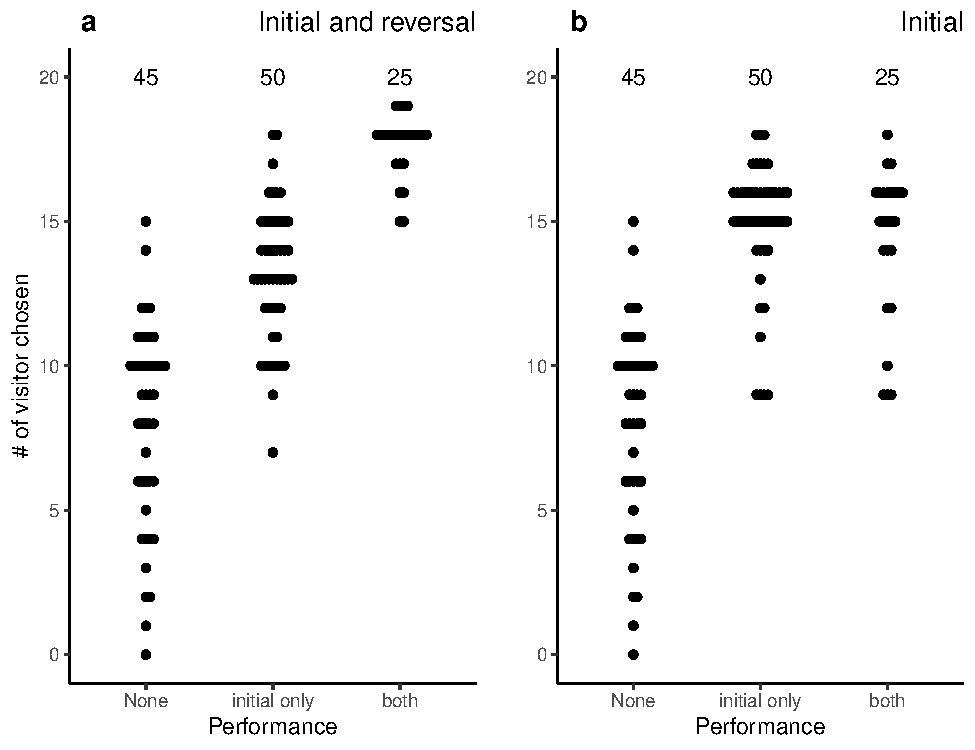
\includegraphics{manuscript_1.0_files/figure-latex/rawdata-1} 

}

\caption{Relation between the response variable used in this study and the
criteria used in previous studies to assess performance in the ephemeral reward
task. In the x axis, we classified the performance of cleaner fish according to
whether they developed a preference for the visitor in the initial round,
in the initial and reversal, or none of them. In the y axis, we add the choices
of two experimental sessions: panel on the left uses one session from the initial
round and one from the reversal round when possible
(as described in the main text); panel on the right uses two sessions from the
initial round for all fish.}\label{fig:rawdata}
\end{figure}








\begin{figure}[H]

{\centering 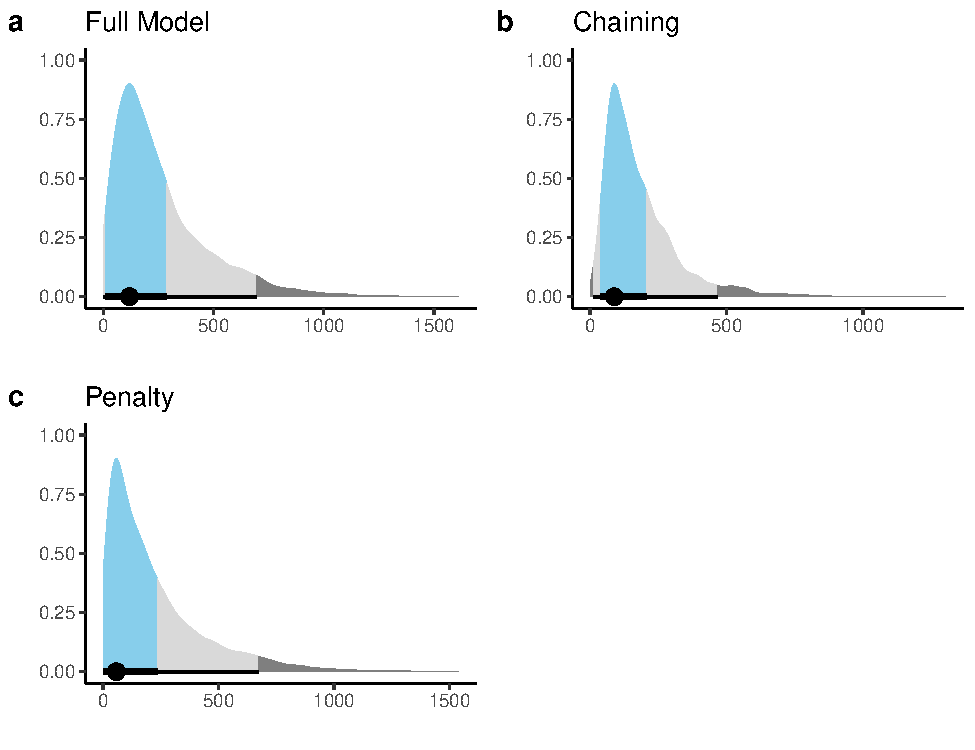
\includegraphics[width=0.95\linewidth,]{manuscript_1.0_files/figure-latex/scaConst-1} 

}

\caption{Posterior distributions for scaling constant for the three model
(``Full model'', chaining only'' and ``penalty only''). We show the kernel
density estimates, below the mode (black dot) and the 65\% (light blue shade)
and 95\% (grey shade) highest posterior density interval. On the top,
panel a shows the posterior distribution from the full model; panel b from
the model with only chaining; and panel c from a model with only penalty.}\label{fig:scaConst}
\end{figure}

\begin{longtable}[]{@{}rc@{}}
\caption{\label{tab:param} Parameter values with which the model was run
in the MCMC. \(\sigma\) refers to the amplitud of the perturbation kernel with the subscript indicating the associated parameter. New values were taken from a uniform distribution. \(\alpha\) refers to the learning rate.}\tabularnewline
\toprule
Parameter & Value \\
\midrule
\endfirsthead
\toprule
Parameter & Value \\
\midrule
\endhead
Learning rounds & 10000 \\
Reward value & 1 \\
\(\alpha\) & 0.05 \\
\(\sigma_{\gamma}\) & 0.3 \\
\(\sigma_{\eta}\) & 4 \\
\(\sigma_{Sca.Const.}\) & 300 \\
Number of chains & 5 \\
Chain lenght & \(1^5\) \\
\bottomrule
\end{longtable}





\begin{verbatim}
## pdf 
##   2
\end{verbatim}

\begin{figure}

{\centering 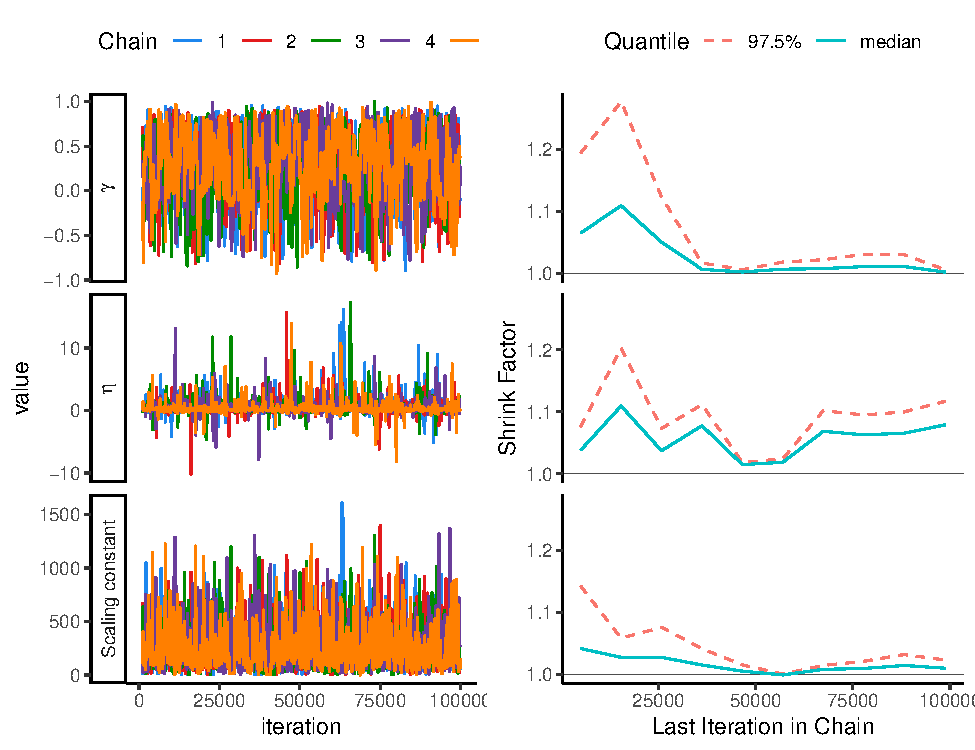
\includegraphics{manuscript_1.0_files/figure-latex/diagnosticsfull-1} 

}

\caption{MCMC convergence diagnostics for the full model.
On the left trace-plots, on the right changes along the chain of the
Gelman and Rubin's shrink factor \citep{brooks_General_1998}.}\label{fig:diagnosticsfull}
\end{figure}





\begin{verbatim}
## pdf 
##   2
\end{verbatim}

\begin{figure}

{\centering 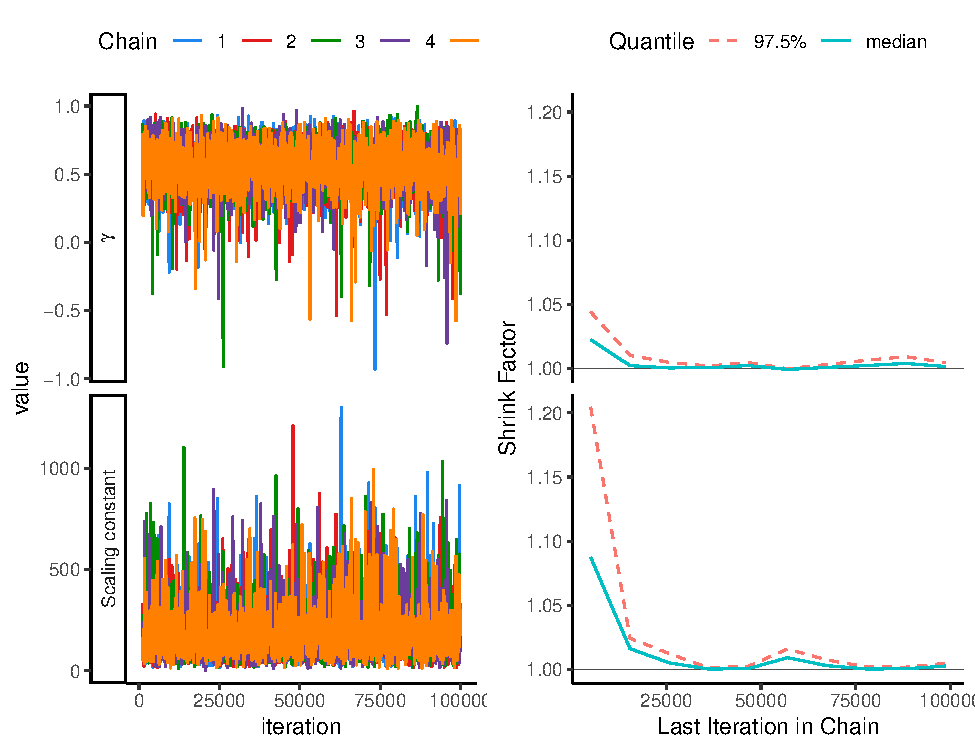
\includegraphics{manuscript_1.0_files/figure-latex/diaggam-1} 

}

\caption{MCMC convergence diagnostics for the chaining model.
On the left trace-plots, on the right changes along the chain of the
Gelman and Rubin's shrink factor \citep{brooks_General_1998}}\label{fig:diaggam}
\end{figure}

\ethics{The Animal Ethics Committee of the Queensland government (DAFF)
approved the project (CA 2016/05/970 and CA 2017/05/1063).}

\dataccess{Please provide details on the data availability.}

\aucontribute{AQ and RB designed the study. ZT collected the data. AQ developed the model and
fitted the model parameters to the data. AQ, RB and ZT wrote the manuscript.}

\competing{The authors declate no conflict of interests.}

\funding{This work was supported by the Swiss National Science Foundation (grants
number: 31003A\_153067/1 and 310030B\_173334/1 to R.B.).}


\ack{ZT and RB kindly thank the staff of Lizard Island Research Station, Dominique
Roche, Sharon Wismer, Olivia Rey,Sandra Ann Binning, Elena Levorato and William McNeely for their
field support. AQ thanks Florian Hartig for statistical advice.}

\bibliographystyle{RS}
\bibliography{Cleanerlearning.bib}


\end{document}
